\chapter{Vector bundles}

\section{Review of linear algebra}

\subsection{The category of vector spaces}

Fix \(\bK\) a field (for this class we only care about \(\bK=\R\)).

Let \(\text{vec}_\bK\) be the category of finite-dimensional \(\bK\) vector spaces:
\begin{itemize}
    \item Objects are (finite dimensional) \(\bK\) vector spaces 
    \item Morphisms are linear maps.
\end{itemize}

The category \(\text{vec}_\bK\) is \dhighlight{abelian}. In particular 
\begin{itemize}
    \item given \(\psi:V\to W\), there exists \[0\to \ker \phi \hookrightarrow V\stackrel{\psi}{\to} W\]
        \[V\stackrel{\psi}{\to} W\to W/\psi(V)\to 0\]
    \item \(V,W\), can form \(V\oplus W \equiv V\times W\) \marginnote{We can only form direct sums of finitely many vector spaces, since \(\text{vec}_\bK\) only contain finite dimensional vector spaces}
\end{itemize}

The category \(\text{vec}_\bK\) is symmetric monoidal:
\begin{align*}
    \text{vec}_\bK \times \text{vec}_\bK \to \text{vec}_\bK\\
    (V,W)\mapsto V \otimes_{\bK} W
\end{align*}

\dhighlight{Note:} \[V\otimes W \simeq W\otimes V\] symmetric and 
\[V\otimes(W\otimes Z)\simeq (V\otimes W)\otimes Z.\]

\dhighlight{Note:} If \(V^1,\dots, V^k\) are vector spaces and \(\{e_j^i\}_{j=1}^l\) basis for \(V^i\), 
then \[\{e_{j_1}^1\otimes\dots\otimes e_{j_k}^k\}\]
basis for \(V^1\otimes \dots\otimes V^k\).

The category \(\text{vec}_\bK\) admits an anti-involution:
\begin{align*}
    (\cdot)^{\vee}:\text{vec}_\bK&\to \text{vec}_\bK^{\text{op}}\\
    V&\mapsto V^\vee \\
    \psi\in\text{hom}(V,W)&\mapsto \psi^\vee \in \text{hom}(W^\vee,V^\vee) \\
    (\cdot)^{\vee\vee} & \equiv \text{id}
\end{align*}

These notions will have corresponding notions for vector bundles.

\subsection{Tensor products}

Recall that the \dhighlight{tensor product} of vector spaces is characterized by:

\dhighlight{Universal property:} If \(\alpha:V^1\times \dots\times V^k\to W\) is a 
multi-linear map, then there exists 
\begin{center}
    \begin{tikzcd}
        \arrow[d,"\pi"]V^1\times \dots \times V^m \arrow[r,"\alpha"]& W\\
        V^1\otimes \dots \otimes V^m \arrow[ru,"\underline{\alpha}\equiv\alpha"]&
    \end{tikzcd}
\end{center}

\begin{definition*}
    Given a vector space \(V\in \text{vec}_\bK\), a \dhighlight{tensor of type} 
    \((k,l)\in \N\times \N\) is an element of 
    \[T^{k,l}V\coloneqq \underbrace{V\otimes \dots \otimes V}_{k\text{ times}}\otimes \underbrace{V^\vee\otimes \dots \otimes V^\vee}_{l\text{ times}}\]   
\end{definition*}

We write \(T^kV\equiv T^{k,0}V\) and \(T^lV^\vee\equiv T^{0,l}V\)

\begin{remark}
    This is not the same as the decomposition into \((l,k)\) forms in complex linear algebra. 
\end{remark}

A tensor \(\alpha\in T^lV^\vee=(T^l V)^\vee\) defines a map \(T^lV\to \bK\), hence also 
a multi-linear map \(V\times \dots\times V\to \bK\). We denote these maps by \(\alpha\) by abuse of notation.

\begin{definition*}
    A tensor \(\alpha\in T^l V^\vee\) is 
    \begin{itemize}
        \item \dhighlight{alternating}: if the induced map \(\alpha:V^1\times \dots\times V^l\to\bK\) satisfies 
            \[\alpha(x_1,\dots,x_i,\dots,x_j,\dots,x_l)=(-1)^{j-i}\alpha(x_1,\dots,x_j,\dots,x_i,\dots,x_l).\]
        \item \dhighlight{symmetric} if the induced map \(\alpha:V^1\times \dots\times V^l\to\bK\) satisfies 
            \[\alpha(x_1,\dots,x_i,\dots,x_j,\dots,x_l)=\alpha(x_1,\dots,x_j,\dots,x_i,\dots,x_l).\]
    \end{itemize}
    We let \(\Lambda^l(V^\vee)\subset T^l V^\vee\) be the subspace of alternating tensors. We let \(\Sigma^lV^\vee\subset T^l V^\vee\)
    be the subspace of symmetric tensors.
\end{definition*}

\markeol{18}

\beginlecture{19}{13.12.2024}

\begin{lemma}\label{lem:8.1}
    \dhighlight{(1):} The inclusion \(\Lambda^k(V^\vee)\subset T^k(V^\vee)\) splits via the map 
    \begin{align*}
        T^k(V^\vee)&\to \Lambda^k(V^\vee)\\
        \alpha&\mapsto \text{alt}(\alpha)\coloneqq \frac{1}{k!}\sum_{\sigma\in S_k}(\text{sgn}(\sigma)) {}^\sigma \alpha
    \end{align*}
    where \[^\sigma \alpha(v_1,\dots,v_k)=\alpha(v_{{\sigma(1)}},\dots,v_{{\sigma(k)}}).\]
    \dhighlight{(2):} The inclusion \(\Sigma^k(V^\vee)\subset T^k(V^\vee)\) also splits via the map 
    \begin{align*}
        T^k(V^\vee)&\to \Sigma^k(V^\vee)\\
        \alpha & \mapsto \text{sym}(\alpha)\coloneqq \frac{1}{k!}\sum_{\sigma\in S_k} {}^\sigma \alpha
    \end{align*}  
\end{lemma}

\begin{proof}\marginnote{We should also check that the maps acutally land in the claimed target set}
    \dhighlight{(1):} We need to show that the composition
    \begin{center}
        \begin{tikzcd}
        \Lambda^k(V^\vee)\arrow[r,"i"] & T^k(V^\vee)\arrow[r,"\text{alt}"] & \Lambda^k(V^\vee)
        \end{tikzcd}
    \end{center}
    is the identity. This is the case because \((\text{sgn}(\sigma)) {}^\sigma\alpha=\alpha\) if \(\alpha \in \Lambda^k(V^\vee)\).

    \dhighlight{(2)} is similar.
\end{proof}

\section{Vector bundles}

\subsection{Basic definitions}

\begin{definition*}
    A (real, smooth) \dhighlight{vector bundle} is a triple \((\pi,E,B)\) where 
    \begin{itemize}
        \item \(E,B\) are manifolds 
        \item \(\pi:E\to B\) is a smooth map
        \item \(E_b=\pi^{-1}(b)\) carries the structure of a real vector space (finite dimensional).\marginnote{If we look at the fibres \dots }
    \end{itemize}
 
    This data must satisfy the following \dhighlight{``local triviality''} condition:

    Given any \(b\in B\), there exists a neighborhood \(b\subset U\) and a diffeomorphism \(\psi^{-1}:\pi^{-1}(U)\simeq U\times V\)
    such that: \marginnote{\(V\) is some real, finite dimensional vector space}
    \begin{enumerate}
        \item[(i)] \(\pi\circ \psi(x,v)=x\)
        \item[(ii)] \(\psi\restrict{E_b}:E_b\stackrel{\simeq}{\to} \{b\} \times V\) is an isomorphism of real vector spaces.  
    \end{enumerate}
    
    \(B\) is called the \dhighlight{base}, \(\pi\) the \dhighlight{projection} and \(E\) is called the \dhighlight{total space}.

\end{definition*}

\begin{remark}
    We assume in this course that \(\text{dim}_\bK(E_b)\) is constant (this is automatic if \(B\) is connected).
    Under this convention we can assume that \(V=\R^k\), since every finite dimensional real vector space is non-cannoically isomorphic to \(\R^k\) for some \(k\in \N\) by composing \(\psi\) with \((\text{id},\phi_V)\), where \(\phi_V\) is said isomorphism.
\end{remark}

\begin{figure}[H]\label{fig:8.1}
    \centering
    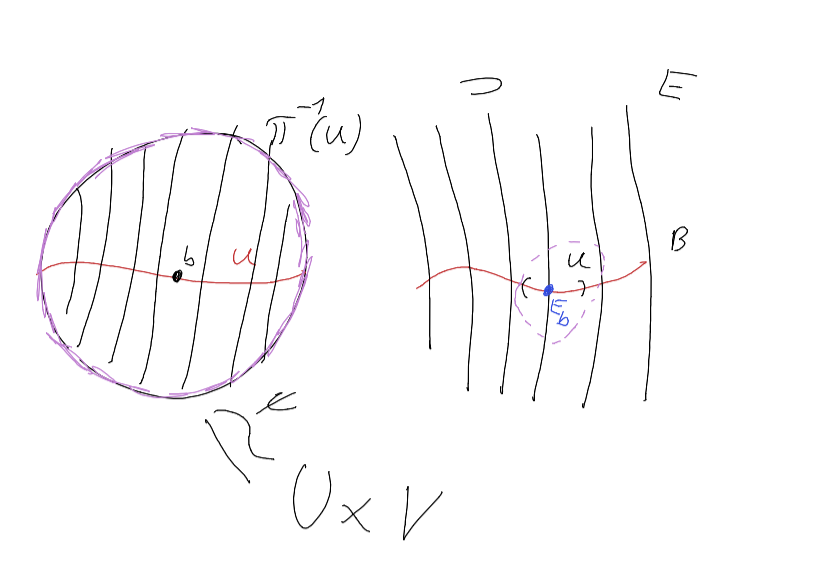
\includegraphics[width=.7\textwidth]{sketch_8_01.png}
    \caption{Sketch 8.01}
\end{figure}
In the homework
\begin{figure}[H]\label{fig:8.2}
    \centering
    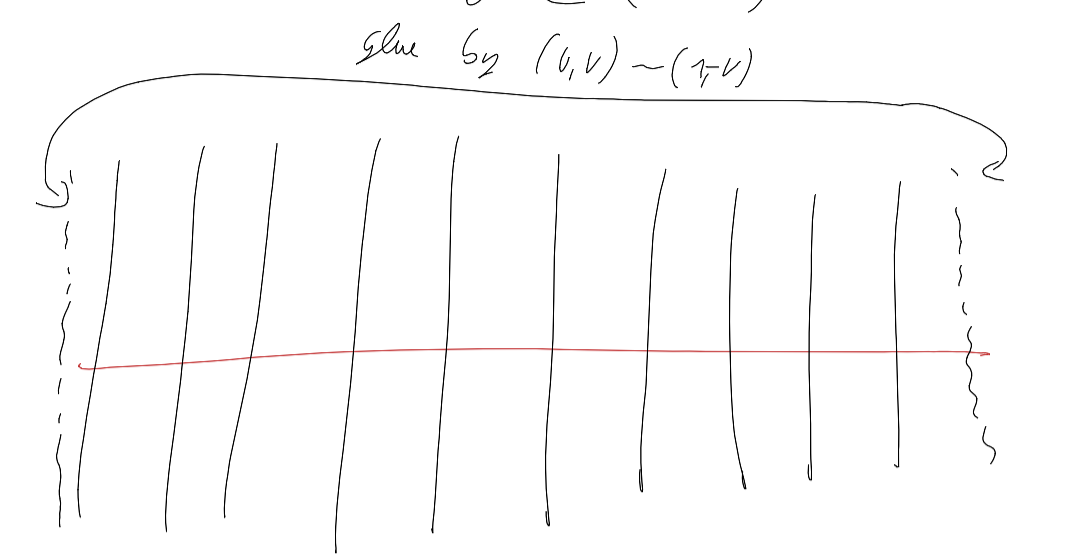
\includegraphics[width=.7\textwidth]{sketch_8_02.png}
    \caption{Sketch 8.02}
\end{figure}
Rigorously \(E:[0,1]\times \R/(0,v)\sim(1,-v)\). Notice that in this case the local triviality really is local, i.e. we can't take \(U=E\).

\begin{definition*}
    A morphism of (smooth, real) vector bundles \((\pi,E,B)\to (\pi',E',B')\) is the data of smooth maps 
    \(F:E\to E',f:B\to B'\) such that 
    \begin{enumerate}
        \item[(i)] \begin{tikzcd}
            \arrow[d,"\pi"] E\arrow[r,"F"] & E'\arrow[d,"\pi'"]\\
            B \arrow[r,"f"] & B'
        \end{tikzcd} commutes. 
        \item[(ii)] \(F\restrict{E_b}:E_b\to E_{f(b)}'\) is a linear map.
    \end{enumerate}
\end{definition*}

\begin{remark} %TODO: Why?
    \(f\) is determined by \(F\) and the condition that \(F\) sends fibers to fibers.\marginnote{Recoverable through quitioning}
\end{remark}

\dhighlight{Notation:} We write \(E=(\pi,E,B), (\pi,E,B)\stackrel{(F,f)}{\to} (\pi',E',B')\) is written as \(F:E\to E'\).

\begin{definition*}
    Given a vector bundle \(E\), a \dhighlight{sub-bundle} is a vector bundle \(F\) over the same base,
    and a map \(i:F\hookrightarrow E\) covering the identity, such that \(F_b\stackrel{i}{\hookrightarrow}E_b\)
    is injective, i.e. 
    \begin{center}
        \begin{tikzcd}
            \arrow[d]F\arrow[r,hook,"i"] & E \arrow[d,"\pi"]\\
            B\arrow[r,"="] & B
        \end{tikzcd}
    \end{center}
    and \(F_b\hookrightarrow E_b\) is injective.
\end{definition*}

\begin{definition*}
    We let \(\text{vectbund}\) be the category whose objects are (smooth, real) vector bundles. We 
    let \(\text{vectbund}(B)\) be the subcategory on vector bundles over \(B\) with morphisms covering the 
    identity.
\end{definition*}

\begin{remark}
    Can similarly set up a theory of \(C^0,C^k,k\geq 1\) vector bundles over \(\R,\C\). This gives rise to 
    analogous categories. Other would therefore write \(\text{vectbund}^\infty\) for what is here jut called \(\text{vectbund}\). 
\end{remark}

\begin{lemma}[Construction]\label{lem:8.2}
    Let \(f:B\to C\) be a smooth map. Then there is a function \(f^\star:\text{vectbund}(C)\to \text{vectbund}(B)\).
    This is called \dhighlight{pullback}. On objects, we have \(f:\underbrace{E}_{\in \text{vectbund}(C)}\to f^*(E)\coloneqq B\times_C E \to B\).
\end{lemma}
\dhighlight{Note:} Here we use the diagram: 
\begin{center}
    \begin{tikzcd}
        \arrow[d,"\pi_B"]f^\star(E)\arrow[r] & E\arrow[d,"\pi"]\\
        B \arrow[r,"f"] & C 
    \end{tikzcd}
\end{center}

\begin{proof}
    Note that \(\pi:E\to C\) is a submersion (always true for vector bundles, follows from the condition \(\pi^{-1}(U)\simeq U\times V\)).
    Hence \(f \pitchfork\pi\)
    are transverse, and the fiber product exists (in the category \(\maninf\)).
    \begin{itemize}
        \item \(\pi_B^{-1}(b)=\pi^{-1}(f(b))\) endows \(\pi_B^{-1}(b)\) with the structure of a vector space
        \item given \(b\in B\) there exist \(U\ni f(b)\), and \(\psi:\pi^{-1}(U)\sim U\times V\). Hence \(\pi_B^{-1}(U)\simeq \pi^{-1}(U)\times V\), which verifies local triviality.
    \end{itemize}

    There is more to check, but the rest is trivial.
\end{proof}

\subsection{Examples of vector bundles}

\begin{example}
    Let \(B=\{x\}\). Then \(\text{vectbund}(\{x\})\simeq \text{vect}_\R\) by 
    \[\{x\}\times V \stackrel{\pi}{\to} \{x\}\mapsfrom V\]
\end{example}

\begin{example}
    Let \(B\) be our favorite smooth manifold. Then there is a unique map \(f:B\to \{x\}\).
    Hence by lemma \ref{lem:8.2}, we have a vector bundle \(f^\star V\). In fact 
    \(f^\star V= B\times V\stackrel{\pi_B}{\to} B\) by \((b,v)\mapsto b\).\marginnote{This is a small exercise}
    Any vector bundle of the form \(f^\star V\) is called \dhighlight{trivial}. 
\end{example}

\begin{remark}
    The Möbius bundle is not trivial:
    \(M\stackrel{\pi}{\to} S^1\), if \(M=S^1 \times \R\to S^1\)  \((x,1)\mapsfrom x\)
    , then we could define a section \(\sigma:S^1\to M,\pi\circ \sigma=\text{id}\) and \(\sigma\neq 0\).
    Contradiction via the intermediate value theorem.
\end{remark}

\begin{example}
    Let \(B\) be any manifold. Then \(TB\stackrel{\pi}{\to} B\) is a vector bundle.
    \marginnote{Given a manifold: is the vector bundle trivial? is a nice question to ask (in the exam?)}
\end{example}

\dhighlight{Exercise:} \(T S^1\simeq S^1\times \R\) 

What about \(TS^2\)?

\subsection{Vector bundles from gluing data}

This gives a mechanism to produce many more examples.

\dhighlight{Construction}: % Own box? 
Let \(M\) be a manifold. Let 
\begin{itemize}
    \item \(\{U_\alpha\}_{\alpha\in \cA}\) be a cover of \(M\)
    \item \(\{V_\alpha\}_{\alpha\in \cA}\) be a collection of vector spaces 
    \item \(\varphi_{\alpha\beta}:U_\alpha\cap U_\beta\to \text{GL}(V_\alpha,V_\beta)\simeq \text{GL}(\R^k)\subset \R^{k^2}\) be 
          smooth maps satisfying \[\varphi_{\alpha\gamma}=\varphi_{\beta\gamma}\varphi_{\alpha\beta}\] on  \(U_\alpha\cap U_\beta\cap U_\gamma\) for all \(\alpha,\beta,\gamma\in\cA\). 
          The equation is called \dhighlight{cocycle condition}.
\end{itemize}
We let \begin{equation}
    E\coloneqq \coprod_{\alpha\in\cA} U_\alpha \times V_\alpha /\sim     
\end{equation}
where \(U_{\alpha}\times V_\alpha \ni (x,v)\sim (x,w)\in U_\beta\times V_\beta\)
if \(w=\varphi_{\alpha\beta}(x)(v)\).

We let \(\pi:E\to M\) be the forgetful map \[[(x,v)]\mapsto x.\]

\begin{lemma}\label{lem:8.3}
    \begin{enumerate}
        \item[(a)] \(\pi:E\to M\) is a vector bundle
        \item[(b)] All vector bundles arise in this way.  
    \end{enumerate}
\end{lemma}

\begin{proof}[Proof sketch]
    \dhighlight{(a)} is obvious (once you believe \(\sim\) is an equivalence relation)

    \dhighlight{(b):} Let \(\pi:E\to B\) be a vector bundle, cover 
    \(B\) by \(\{U_\alpha\}\), \(\psi:\pi^{-1}(U_\alpha)\to U_\alpha\times V_\alpha\) and let \(\varphi_{\alpha,\beta}=\psi_\beta\circ \psi_\alpha^{-1}\). \qedhere 
\end{proof}

\markeol{19}

\beginlecture{20}{17.12.2024}

\dhighlight{Terminology:} A vector bundle \(\pi:E\to B\) has to satisfy the local triviality condition: around any \(p\in B\exists U\ni o\land \psi_U:\pi^{-1}(U)\simeq U\times V\),
where \(V\) is a vector field. \(\psi:U\) is called a \dhighlight{local trivialization}. We call 
\(E_b,\in B\) the \dhighlight{fibers}. \marginnote{and the \(E_b\) trivially are vector spaces}
\((U\cap \mathcal{V})\times V_U \to (U\cap \mathcal{V})\times V_{\mathcal{V}}\) by the transition function 
\(\psi_\mathcal{V}\circ \psi_{U}^{-1}\)

\[(x,v)\mapsto (x,w)=(x,\psi_\mathcal{V}\circ \psi_{U}^{-1}(x,v)).\]
\marginnote{The transition function only really acts on the second component}
\begin{remark}
    If the instructor had different taste, the above construction might as well have been the definition
\end{remark}

\begin{remark}
    \begin{itemize}
        \item Different choices of data \((\{U_\alpha\},\{V_\alpha\},\{\phi_{\alpha\beta}\})\) may give rise to 
              the same vector bundle. \marginnote{For example, if you take more open sets, you still get the same structure}    
        \item however, with appropriate notion of equivalence, \{vector bundles\} \(\equiv (\{U_\alpha\},\{V_\alpha\},\{\phi_{\alpha\beta}\})\).
              This can be made precise by defining a category of gluing data, which then becomes equivalent to the category of vector bundles. 
    \end{itemize}
\end{remark}

\section{Globalizing linear algebra constructions}

\begin{theorem}[Omnibus theorem]\label{thm:8.4}\marginnote{Not really well defined ...}
    Any  canonical linear algebra construction can be globalized 
    to the category of smooth vector bundles. 

    More precisely: The category \(\text{vectbund}_\R\) admits 
    \(\cdot \oplus \cdot,\cdot \otimes \cdot,(\cdot)^\vee,(\cdot)/(\cdot), \text{Hom}(\cdot,\cdot),\dots\)

    \begin{enumerate}
        \item[(i)] the operations are compatible with pullback: i.e. given \(f:B\to B'\),
        \[f^\star(E'\oplus F')=f^\star(E')\oplus f^\star(F').\]
        Also \(f^\star(E'\otimes F')=f^\star(E')\otimes f^\star(F')\) for \(E'\to B'\) and \(F'\to B'\).  
        \item[(ii)] On \(\text{vectbund}_\R(\{x\})\simeq \text{vect}_\R\), the operations coincide. 
    \end{enumerate}
\end{theorem}

\begin{remark}[Warning]
    In contrast to \(\text{vect}_\bK\), the category \(\text{vectbund}_\R\) is \dhighlight{not abelian} (nor is 
    \(\text{vectbund}(B)\) in general). To see  what goes wrong:

    Consider \((E=\R\times \R)\to \R\); \(\phi:\R\times \R \to \R\times \R\), \marginnote{first component is the base}
    \[(t,v)\mapsto (t,tv).\]
    Note: \(\phi_t:\underbrace{E_t}_{=\R}\to E_t, v\mapsto tv\). If \(t\neq 0\), then \(\phi_t:E_t\to E_t\)
    is an isomorphism. If \(t=0,\phi_t\equiv 0\) (not an isomorphism).
    
    So \(\text{ker}(\phi)\) \textit{wants to be}
    \begin{figure}[H]\label{fig:8.03}
        \centering
        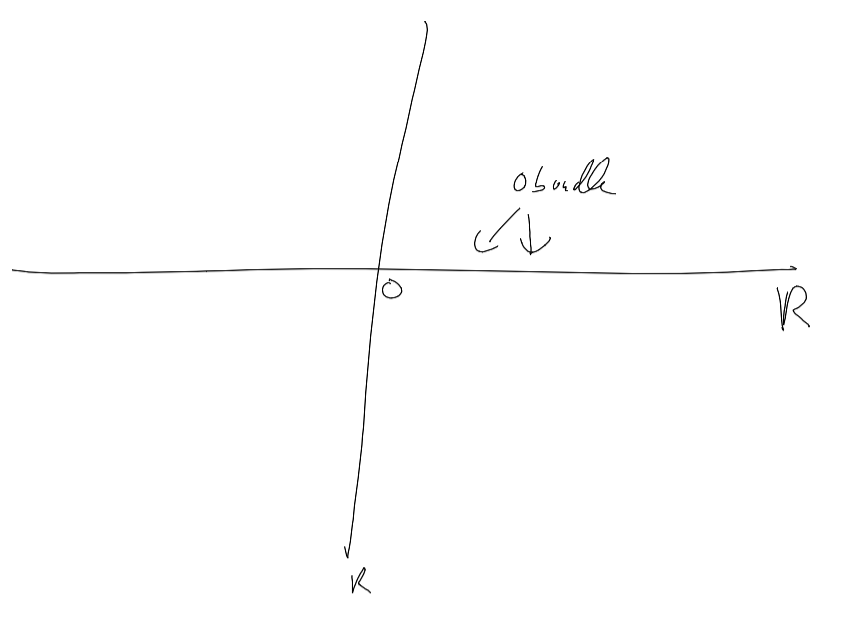
\includegraphics[width=.7\textwidth]{sketch_8_03.png}
        \caption{Sketch 8.03}
    \end{figure}
    The \textit{fix} is to embed \(\text{vectbund}_\R\subset\text{sheaves}_\R\). 
    This is the start of a long story \dots 
\end{remark}

\begin{remark}[Warning]
    In this category \(\text{vectbund}_\R\) there is a difference between 
    \dhighlight{sub-bundles} and \dhighlight{sub-objects}. 
    We say that \begin{tikzcd}
        \arrow[rd]E\arrow[rr,hook,"i"] && F\arrow[ld]\\
        &B&
    \end{tikzcd}
    is a sub-bundle, if \(i_b:E_b\to F_b\) is injective.

    Meanwhile, in any category, a sub-object \(C\) of \(D\) is a map \(C\to D\), which is a 
    \dhighlight{monomorphism} (this means that for all \(Z\), \begin{tikzcd}
    Z\arrow[r,bend right,"f_1"]\arrow[r,bend left,"f_2"]&C\
    \end{tikzcd}
    \(i\circ f_1=i\circ f_2\implies f_1=f_2\)).
    
    We can only form quotients of sub-bundles. In fact \(\phi\) from the previous example is a 
    sub-object, but not a sub-bundle.
\end{remark} 

The omnibus theorem allows us to produce new bundles from old:
\begin{example}
    \begin{center}
        \begin{tikzcd}
            &T^\star M \arrow[d,"="]& \arrow[ld,"="]\coloneqq U_{m\in M} (T_m M)^\vee\\
            TM\arrow[ru] & (TM)^\vee 
        \end{tikzcd}
    \end{center}
    the cotangent bundle and 
    \begin{center}
        \begin{tikzcd}
            &\Lambda^k T^\star M\\
            TM\arrow[ru]\arrow[rd] & \\
            &\Sigma^k T^\star M 
        \end{tikzcd}
    \end{center}
    which are the \dhighlight{k-th exterior power of the cotangent bundle} and the \dhighlight{k-th symmetric power of the cotangent bundle}.
\end{example}

\begin{proof}[Proof of theorem \ref{thm:8.4}]
    \phantom{Test}

    \begin{displayquote}[Prof. Côté]
        Proof: These definitions are all natural, so how could they fail?
    \end{displayquote}

    In (slightly) more detail: Let \(E^1,\dots,E^k\) be vector bundles over \(B\).
    Let \(\{U_\alpha\}\) be an open cover of \(B\), which simultaneously trivializes all of the \(E^i\).
    Then the \(E^i\) cna be presented as follows: 
    \begin{itemize}
        \item \(\{V_\alpha^i\}_{\alpha\in\cA}\)
        \item \(\{\phi_{\alpha\beta}^i:U_\alpha\cap U_\beta\to \text{GL}(V_\alpha^iV_\beta^i)\}\), such that \(\phi_{\alpha\gamma}=\phi_{\beta\gamma}\phi_{\alpha\beta}\) (lemma \ref{lem:8.3}).
    \end{itemize} 
    Let \(\mathfrak{F}(E^1\dots,E^k)\in\text{vectbund}_\R(B)\) defined by applying some combination of 
    \(\oplus,\otimes,\text{Hom}(\cdot,\cdot),(\cdot)/(\cdot),\dots\) (any cannoical linear algebraic construction) fiberwise.

    I.e. \(\mathfrak{F}(E^1,\dots,E^k)\coloneqq \bigcup_{b\in B}\mathfrak{F}(E_b^1,\dots,E_b^k)\)\marginnote{the fibers are all disjoint}

    We can present \(\mathfrak{F}(E^1,\dots,E^k)\) by 
    \begin{itemize}
        \item \(\{\mathfrak{F}(V_\alpha^1,\dots,V_\alpha^k)\}_{\alpha\in \cA}\)
        \item \(\phi_{\alpha\beta}:U_\alpha\cap U_\beta \to \text{GL}(\mathfrak{F}(V_\alpha^1,\dots,V_\alpha^k),\mathfrak{F}(V_\beta^1,\dots,V_\beta^k))\)
    \end{itemize}

    Must check: Smoothness of the \(\phi_{\alpha\beta}^i\) implies smoothness of \(\phi_{\alpha\beta}\). This 
    is essentially because, of the  fixing \(V_\alpha^i\simeq \R^k\), then \(\phi_{\alpha\beta}^i\) is just 
    a matrix and \(\phi_{\alpha\beta}(x)\) is obtained from \(\{\phi_{\alpha\beta}^i\}\) by a sequence of matrix addition, multiplications,
    taking adjoints, \dots all of which preserve smoothness of the coefficients. \qedhere

\end{proof}

\section{Sections of vector bundles}

\begin{definition*}
    Let \(\pi:E\to B\) be a vector bundle. A \dhighlight{Section} \(\sigma:B\to E\) is a 
    smooth map, such that \(\pi\circ \sigma=\text{id}\).
\end{definition*}
We let \(\Gamma(E)\) denote the space of sections of \(E \to M\). \marginnote{Here \(M=B\) will be switched arbitrarily}

\begin{lemma}\label{lem:8.5}
    \begin{enumerate}
        \item[(i)] \(\Gamma(E)\) is an \(\R\)-vector space 
        \item[(ii)] \(\Gamma(E)\) is a module over \(C^\infty(M,\R)=C^\infty(M)\)  
    \end{enumerate}
\end{lemma}

\begin{proof}
    Exercise. Same proof as for \(TM\).
\end{proof}

These are very important definitions!

\begin{example}
    \(E=TM\to M,\Gamma(E)=\cX(M)\), elements are called \dhighlight{vector fields}.
\end{example}

\begin{example}\marginnote{1-forms are dual to vector fields}
    \(E=T^\star M\to M,\Gamma(E)\eqqcolon \Omega^1(M)\), elements are called \dhighlight{1-forms}.
\end{example}

\begin{example}
    \(E=\Lambda^k T^\star M \to M\), \(\Gamma(\Lambda^k T^star M)\eqqcolon \Omega^k(M)\), elements are called \dhighlight{k-forms}
\end{example}

\begin{example}\marginnote{A little silly, but good to see}
    \(E=M\times \R^k\to M, \Gamma(E)\equiv C^\infty(M,\R^k)\)
    He wrote: %TODO: Fix
    \[\Gamma(E)\ni\sigma\mapsto (x\mapsto (x,\sigma_x(x)))\]
    But erased it later, to be fixed. Essentially the point is that the second component describes the function.
\end{example}

\begin{remark}
    \(\Gamma(E)\) is an infinite dimensional vector space (unless \(E=M\times \{x\}\)).
\end{remark}

\begin{lemma}\label{lem:8.6}
    Let \(\pi:E\to B\) be a vector bundle. Suppose that \(A\subset B\) is closed. Let \(A\subset U\) be open.
    Suppose that \(\sigma:A\to E\) is a smooth section (i.e. around every \(a\in A,\sigma\) extends to a smooth section in a neighborhood of \(a\)).
    
    Then there exists \(\tilde{\sigma}\in \Gamma(E)\) such that 
    \begin{enumerate}
        \item[(i)] \(\tilde{\sigma}\restrict{A}=\sigma\)
        \item[(ii)] \(\text{supp}(\tilde{\sigma})\subset U\)  
    \end{enumerate}
\end{lemma}

\begin{proof}
    Sheet 12. We already have a lemma for the trivial case, then use partition of unity.
\end{proof}

Picking a section to a point, we can globally extend it to a smooth function, then we can easily connect it 
to the previous remark.

\markeol{20}

\beginlecture{21}{20.12.24}

\begin{definition*}
    Let \(f:M\to M'\) be a smooth map. Let 
    \(\pi:E'\to M'\) be a vector bundle over \(M'\). Then 
    there is a \(\R\) linear map
    \begin{align*}
        \Gamma(E')&\to \Gamma(f^\star(E'))
        \sigma & \mapsto \sigma \circ f = f^\star \sigma
    \end{align*}
    i.e. 
    \begin{center}
        \begin{tikzcd}
            \arrow[d]f^\star E'\arrow[r] & E' \arrow[d,swap,"\pi'"]\\
            \arrow[u,bend left,"\sigma\circ f"]M \arrow[r,"f"]& M' \arrow[u,bend right,swap, "\sigma"]
        \end{tikzcd}
    \end{center} 
    If \(E'=T^\star M'\), then we have 
    \begin{center}
        \begin{tikzcd}
            \arrow[d]T^\star M & \arrow[l,"df^\vee"]\arrow[d]f^\star (T^\star M')\arrow[r] & T^\star M'\arrow[d]\\
            \arrow[u,bend left,"df^\vee\circ \sigma \circ f"]M \arrow[r,"="] & M \arrow[r,"f"]& M' \arrow[u,bend right, swap, "\sigma"]
        \end{tikzcd}
    \end{center}
    where all vertical maps are projections.
    Here \(df^\vee(p,v)=(p,df_p^\vee(v))\) for \(p\in M,v\in f^\star(T^\star M')_p=T_{f(p)}^\star M'\)
    By abuse of notation we also write 
    \[f^\star \sigma=df^\vee\circ \sigma \circ f\in \Gamma(T^\star M)=\Omega^1(M).\]
\end{definition*}

The \dhighlight{upshot} is that we can pullback 1-forms along smooth maps.

{\color{red} In contrast, we can not push forward vector fields along arbitrary smooth maps.}\marginnote{We have already seen examples, but it is obvious, since we can't reverse the projection maps \dots}

Concretely: if \(\sigma \in \Omega^1(M')\), then \(f^\star \sigma\in \Omega^1(M)\) is 
characterized by the formula
\marginnote{This is the only thing that can make sense}
\[(f^\star \sigma)_p(\underbrace{v}_{T_pM})=\sigma_{f(p)}(df_p(v)).\]
More generally, if \(\sigma \in \Gamma(T^k T^\star M'), f^\star\in  \gamma(T^k T^\star M)\)
is characterized by the formula 
\[(f^\star \sigma)_p(v_1,\dots,v_k)=\sigma_{f(p)}(df_p(v_1),\dots,df_p(v_k)).\]

\begin{definition*}
    Let \(\pi:E\to M\) be a vector bundle. Let \(X^1,\dots,X^k\in \Gamma(E)\) (assuming that the fibers have dimension \(k\)).
    We say: 
    \begin{enumerate}
        \item[(1)] \(X^1,\dots,X^k\) is a \dhighlight{local frame} at \(p\in M\), if \(\text{span}(X^1(p),\dots,X^k(p))=E_p\)
        \item[(2)]  \(X^1,\dots,X^k\) is a \dhighlight{global frame}, if \(\text{span}(X^1(q),\dots,X^k(q))=E_q,\forall q\in M\)
    \end{enumerate}
\end{definition*}

\dhighlight{Exercise:} If \(X^1,\dots, X^k\) is a local / global frame for \(E\stackrel{\pi}{\to}M\), then 
\((X^{1})^\vee,\dots,(X^{k})^\vee\) is a local / global frame for \(E^\vee \to M\), hence \(((X^i(p))^\vee)(X^j(p))=\delta_{ij}\).

\begin{example}
    For \(M=\R^n\) we have \(\{\partial_{x_1},\dots,\partial_{x_n}\}\) a global frame and we write 
    \(dx_i=(\partial_{x_i})^\vee\).
\end{example}